%\begin{titlepage}
\chapter*{}
\pagestyle{plain}

\begin{center}
\Huge{\textsc{Anexos}}
\end{center}

\addcontentsline{toc}{chapter}{Anexos}
%\end{titlepage}

\chapter*{}

\pagestyle{myheadings}
\markboth{ANEXOS}{ANEXO A}

\addcontentsline{toc}{section}{Anexo A: C�digo fuente}
\section*{Anexo A: C�digo fuente}
\subsection*{Clase para permitir movimiento aut�nomo al robot}
\lstinputlisting[language=c++, title={BaseCon.cpp}]{BaseCon.cpp}

\subsection*{Clase con la funci�n de reconocer obst�culos en el plano}
\lstinputlisting[language=c++, title={Blobs.cpp}]{Blobs.cpp}
\lstinputlisting[language=c++, title={Blobs.hpp}]{Blobs.hpp}

\subsection*{Clase que representa al sensor MPU6050}
Esta clase se ocupa de inicializar al sensor y obtener los �ngulos de inclinaci�n del Robot.
\lstinputlisting[language=c++, title={Giro.cpp}]{Giro.cpp}

\subsection*{Utilitarios}
En este archivo se encuentran las funciones \texttt{calcular\_distancia()} y \texttt{calcular\_distancia\_horizontal()}, que calculan la distancia vertical y horizontal de un objeto detectado en el plano. Tambi�n se encuentra la funci�n \texttt{leerConfigFile()}, que sirve para leer archivos de configuraci�n.

\lstinputlisting[language=c++, title={Utils.cpp}]{Utils.cpp}

\markboth{ANEXOS}{ANEXO B}
\addcontentsline{toc}{section}{Anexo B: Fotos del Robot}
\section*{Anexo B: Fotos del Robot}
%Robot con todos sus componentes instalados.

\begin{figure}
    \centering
    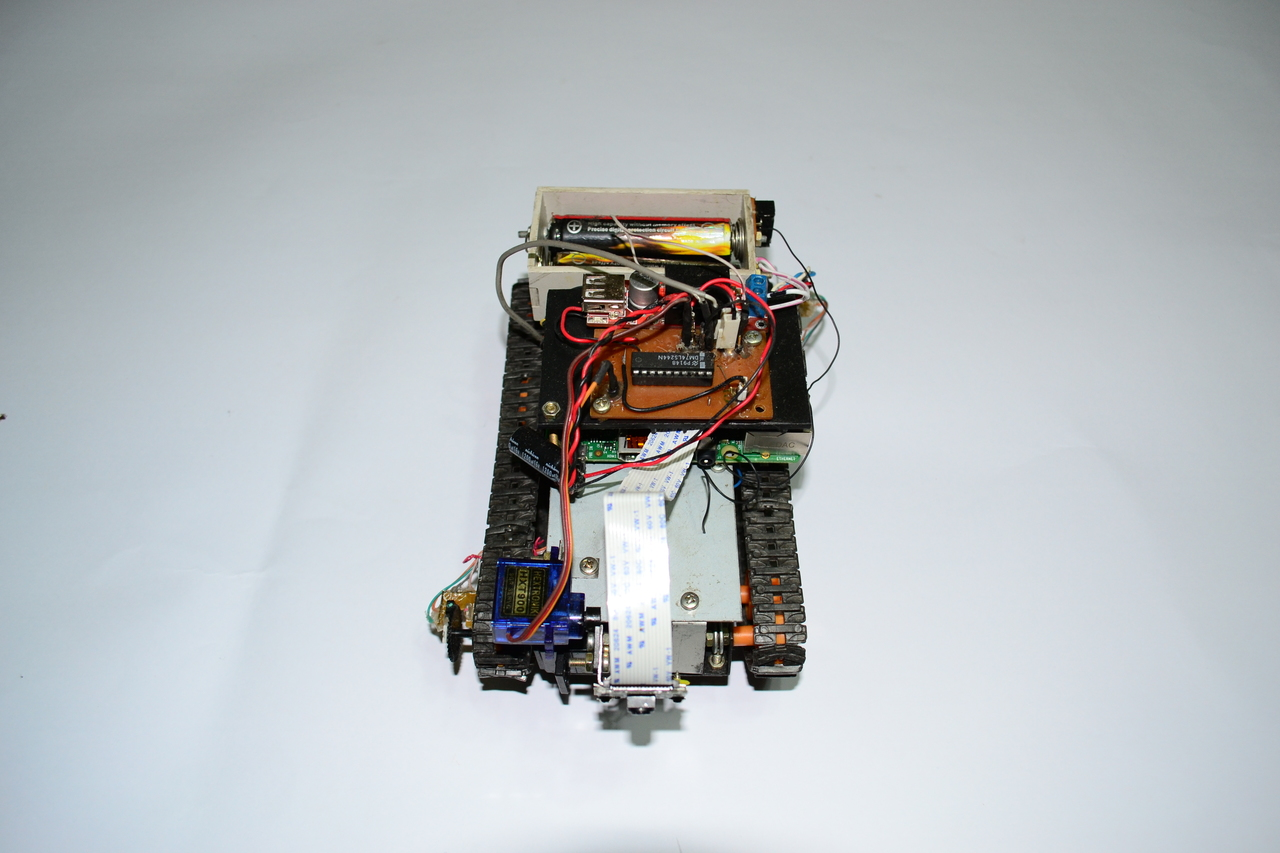
\includegraphics[width=0.8\textwidth]{r-DSC_0009.JPG}
    \caption{Vista frontal del robot. Se observa: el distribuidor de energ�a y regulador de voltaje al centro.}
\end{figure}

\newpage
\markboth{ANEXOS}{ANEXO C}
\addcontentsline{toc}{section}{Anexo C: Planilllas de seguimiento de sprint}
\section*{Anexo C: Planilllas de seguimiento de sprint}
\input{021-Anexos-SeguimientoSprintA.tex}
\input{022-Anexos-SeguimientoSprintB.tex}
\input{023-Anexos-SeguimientoSprintC.tex}
\input{024-Anexos-SeguimientoSprintD.tex}
\input{025-Anexos-SeguimientoSprintE.tex}
\input{026-Anexos-SeguimientoSprintF.tex}
\input{027-Anexos-SeguimientoSprintG.tex}
